%=============================================================================%
% Author: Pablo S�nchez                                                       %
%        (p.sanchez@unican.es http://personales.unican.es/sanchezbp)          %                                                                               %                                                                             %
% Section : Main File                                      Date: 23/02/2011   %
% Version : 1.0                                                               %                                                                             %                                                                             %
% Conference: SPLC 2011                                                       %
%=============================================================================%

\documentclass[10pt, conference, compsocconf]{IEEEtran}

\IEEEoverridecommandlockouts

\usepackage{graphicx}
\usepackage{amsfonts}
\usepackage{color}

\newcommand{\imp}[1]{{\small \sf #1}}
\newcommand{\todo}[1]{\color{red} TODO: #1 \color{black}}

\begin{document}
%
% paper title
% can use linebreaks \\ within to get better formatting as desired
\title{Analysis of Constraints including Clonable Features using Hydra
\thanks{This work has been supported by the Spanish Ministry Project TIN2008-01942/TIN, the EC STREP Project AMPLE IST-033710 and the Junta de Andaluc{\'i}a regional project FamWare TIC-5231}}

\author{
\IEEEauthorblockN{Pablo S\'{a}nchez}
\IEEEauthorblockA{Dpto. Matem\'{a}ticas, Estad\'{i}stica y Computaci\'{o}n  \\
Universidad de Cantabria \\
Santander (Cantabria, Spain) \\
p.sanchez@unican.es}
\and
\IEEEauthorblockN{Jos\'{e} Ram\'{o}n Salazar, Lidia Fuentes}
\IEEEauthorblockA{
Dpto. Lenguajes y Ciencias de la Computaci\'{o}n \\
Universidad de M\'{a}laga \\
M\'{a}laga (M\'{a}laga, Spain) \\
\{salazar, lff\}@lcc.uma.es}
}

\maketitle

\begin{abstract}
	%===============================================================================%
% Author: Pablo S�nchez (pablo@lcc.uma.es; http://www.lcc.uma.es/~pablo)        %
% Section : Abstract                                     Date: 19/11/2009       %
% Version : 1.0                                                                 %
% Conference: TOOLS 2010                                                        %
%===============================================================================%

% The addition of clonable features to feature models have increased the
% expressiveness of feature models, allowing the modelling of structural
% variability. Using clonable features we can model that, for instance, automated
% houses have a variable number of floors and rooms. Nevertheless, clonable
% features create new research challenges. Currently, some  state-of-art feature modelling tools are able to model and configure clonable features. But, as the experienced reader probably knows, it is not always possible to express all the relationships between features using feature models. As a consequence, the the definition of external constraints, such as mutual exclusion between features, is often required. Nevertheless, the semantics of these state-of-art feature constraints become undefined when they are applied to clonable features. In order to overcome this limitation, this paper presents a new language for specifying external constraints between features, which supports clonable features. We also explain how to automatically determine if a given selection of features satisfies the constraints expressed in this new language by means of translating these constraints into a Constraint Satisfaction Problem (CSP). We validate our ideas by applying them to a SmartHome software product line provided by Siemens AG.

Clonable features increase the expressiveness of traditional feature models, allowing the modelling of structural variability. Using clonable features, we can specify, for instance, automated houses have a variable number of floors and rooms.  it is not always possible to express all the relationships between features using feature models. For instance, in a feature model for a SmartHome, a feature like Presence Simulation might require the selection of an Automatic Lights features. As a consequence, the definition of external constraints, such as A implies B, to capture these relationships is often required. Nevertheless, the semantics of these state-of-art external constraints become undefined when they are applied to clonable features. To overcome this limitation, this paper presents: (1) a new language for specifying external constraints involving clonable features; and (2) an automatic reasoner, which transform these constraints into a Constraint Satisfaction Problem (CSP), in order to analyse them. We validate our ideas by applying them to a SmartHome industrial software product line.

%Traditional feature models are not enough for modelling 
\end{abstract}

\begin{IEEEkeywords}
Feature Models, Clonable Features, Constraint Analysis
\end{IEEEkeywords}

\section{Introduction}
\label{sec:introduction}

%==================================================================%
% Author : Doe Doe, John                                           %
%          S�nchez Barreiro, Pablo                                 %
% Version: 1.0, dd/mm/yyyy                                         %                   %                                                                  %
% Memoria del Proyecto Fin de Carrera                              %
% Introducci�n, archivo ra�z                                       %
%==================================================================%

%%% Schema to write a paper introduction
%% Description of Purpose
	% What problem, issue or question does this research address ?
		%
	% What limitations or failings of current understanding, knowledge, method,
	% or technologies does this research resolve ?
		%
	% What is the significance of the problem issue or question ?
		%
%% Goal statement
	% What new understanding, knowledge, methods or technologies will this
	% research generate ?
		%
	% How this address the purpose of the work ?
		%
%% Approach
	% What experiments, prototypes or studies will be done to achieve the stated % goal ?
		%
	% How will achievement or contribution of the research be demonstrated or validated ?
		%

\chapterheader{Introduction}{Introduction}
\label{chap:introduction}

% Introducci�n al cap�tulo

\chaptertoc

\section{Introducci�n}
\label{sec:intr:introduction}

TODO: Siguiendo el esquema que aparece arriba, escribir la introducci�n

\section{Motivaci�n and Contribuciones}
\label{sec:intr:motivation}

TODO: Esta secci�n es m�s para tesis doctorales que para proyectos fin de carrera. La dejamos de momento pero se podr�a eliminar

\section{Visi�n General del Proyecto}
\label{sec:intr:overview}

TODO: Esto est� bien dejarlo, pero tambi�n es suprimible

\section{Estructura del Documento}
\label{sec:intr:organization}

Esto es una especie de �ndice ampliado y se deja, suele ser bastante �til para que el que est� vago se lea esto y se acabe el problema.







\section{Motivation}
\label{sec:motivation}

%===============================================================================%
% Section :                                      Date: 19/11/2009               %
% Version : 1.0                                                                 %
% Conference: Caise 2010                                                        %
%===============================================================================%

This section firstly introduces clonable features~\cite{czarnecki:2005d,czarnecki:2005} and explains the concepts and ideas behind them. Then, we explain why clonable features are important. Finally, we identify the research challenges created by clonable features.

\subsection{Background: clonable features}

%%==================================================================%%
%% Author : Tejedo Gonz�lez, Daniel                                 %%
%%          S�nchez Barreiro, Pablo                                 %%
%% Version: 1.0, 18/11/2012                                         %%                   %%                                                                  %%
%% Memoria del Proyecto Fin de Carrera                              %%
%% Antecedentes, archivo ra�z                                       %%
%%==================================================================%%

\chapterheader{Antecedentes}{Antecedentes}
\label{chap:background}

Este cap�tulo trata de describir a grandes rasgos las t�cnicas, tecnolog�as y herramientas utilizadas para el desarrollo del presente Proyecto Fin de Carrera. En primer lugar, se introducir� el caso de estudio que se utilizar� de forma recurrente a lo largo del proyecto, que es una l�nea de productos software para software de control para hogares inteligentes. Para ello se describen en primer lugar diversos conceptos relacionados al dominio del proyecto, como son las l�neas de productos software y los �rboles de caracter�sticas. A continuaci�n, se describen dos principales herramientas de Ingenier�a de Lenguajes Dirigida por Modelos utilizadas: \emph{Ecore} y \emph{EMFText}. Por �ltimo, se describe brevemente la arquitectura de plugins de Eclipse, dado que nuestro proyecto deb�a integrarse en dicho entorno.

\chaptertoc

\section{Caso de Estudio: Software para Hogares Inteligentes}
\label{sec:back:spl}
%%==================================================================%%
%% Author : Perez Ruiz, Alejandro                                   %%
%% Author : Pablo S�nchez                                           %%
%% Version: 1.1, 13/06/2011                                         %%
%%                                                                  %%
%% Memoria del Proyecto Fin de Carrera                              %%
%% Planificacion/CasoEstudio                                        %%
%%==================================================================%%

El objetivo �ltimo del presente proyecto es la construcci�n de una l�nea de productos software sobre la plataforma .NET para hogares automatizados y/o inteligentes.

%%===========================================================================%%
%% NOTA(Pablo): Dado el contexto del proyecto, este p�rrafo no interesa      %%
%%===========================================================================%%
%%
%% Se ha elegido este dominio de aplicaci�n por ser un dominio donde el uso
%% de un enfoque basado en L�neas de Productos Software se hace casi
%% imperativo, debido a la gran variabilidad existente en estos productos.
%% Esta  variabilidad se debe tanto a motivos de hardware, dado que los
%% dispositivos a ser controlados e interconectados pueden variar enormemente,
%% como funcionales, dado que existen multitud de funcionalidades que se pueden
%% ofrecer de manera opcional o alternativa al usuario, no siendo necesario que
%% un determinado hogar las posea todas ellas.
%%
%%===========================================================================%%

El objetivo de estos hogares es aumentar la comodidad y seguridad de sus habitantes, as� como hacer un uso m�s eficiente de la energ�a consumida. Los ejemplos m�s comunes de tareas automatizadas dentro de un hogar inteligente son el control de las luces, ventanas, puertas, persianas, aparatos de fr�o/calor, as� como otros dispositivos, que forman parte de un hogar. Un hogar inteligente tambi�n busca incrementar la seguridad de sus habitantes mediante sistemas automatizados de vigilancia y alerta de potenciales situaciones de riesgo. Por ejemplo, el sistema deber�a encargarse de detecci�n de humos o de la existencia de ventanas abiertas cuando se abandona el hogar.

El funcionamiento de un hogar inteligente se basa en el siguiente esquema: (1) el sistema lee datos o recibe datos de una serie de sensores; (2) se procesan dichos datos; y (3) se activan los actuadores para realizar las acciones que correspondan en funci�n de los datos recibidos de los sensores.

Todos los sensores y actuadores se comunican a trav�s de un dispositivo especial denominado puerta de enlace (\emph{Gateway}, en ingl�s). Dicho dispositivo se encarga de coordinar de forma adecuada los diferentes dispositivos existentes en el hogar, de acuerdo a los par�metros y preferencias especificados por los habitantes del mismo. Los habitantes del hogar se comunicar�n con la puerta de enlace a trav�s de una interfaz gr�fica.
Este proyecto tiene como objetivo el desarrollo de un hogar inteligente como una l�nea de productos software, con un n�mero variable de plantas y habitaciones. El n�mero de habitaciones por planta es tambi�n variable. La l�nea de productos deber� ofrecer varios servicios, que podr�n ser opcionalmente incluidos en la instalaci�n del software para un un hogar determinado. Dichos servicios se clasifican en funciones b�sicas y complejas, las cuales describimos a continuaci�n.

\paragraph{Funciones b�sicas} \ \\

\begin{enumerate}
\item \emph{Control autom�tico de luces:} Los habitantes del hogar deben ser capaces de encender, apagar y ajustar la intensidad de las diferentes luces de la casa. El n�mero de luces por habitaci�n es variable. El ajuste debe realizarse especificando un valor de intensidad.
\item \emph{Control autom�tico de ventanas:} Los residentes tienen que ser capaces de controlar las ventanas autom�ticamente. De tal modo que puedan indicar la apertura de una ventana desde las interfaces de usuario disponibles.
\item \emph{Control autom�tico de persianas:} Los habitantes podr�n subir y bajar las persianas de las ventanas de manera autom�tica.
\item \emph{Control autom�tico de temperatura:} El usuario ser� capaz de ajustar la temperatura de la casa. La temperatura se medir� siempre en grados celsius.
\end{enumerate}

\paragraph{Funciones complejas} \ \\

\begin{enumerate}
\item \emph{Control inteligente de energ�a:} Esta funcionalidad trata de coordinar el uso de ventanas y aparatos de fr�o/calor para regular la temperatura interna de la casa de manera que se haga un uso m�s eficiente de la energ�a. Por ejemplo, si se recibe la orden de calentar la casa, a la vez que se activan los radiadores se cerrar�n las ventanas para evitar las p�rdidas de calor.
\item \emph{Presencia simulada:} Para evitar posibles robos, cuando los habitantes abandonen la casa por un periodo largo de tiempo, se deber� poder simular la presencia de personas en las casas. Hay dos opciones de simulaci�n (no exclusivas):
	\begin{enumerate}
	\item \emph{Simulaci�n de las luces:} Las luces se deber�n apagar y encender para simular la presencia de habitantes en la casa.
	\item \emph{Simulaci�n de persianas:} Las persianas se deber�n subir y bajar autom�tica para simular la presencia de individuos dentro de la casa.
	\end{enumerate}
\end{enumerate}

Todas estas funciones son opcionales. Las personas interesadas en adquirir el sistema podr�n incluir en una instalaci�n concreta de este software el n�mero de funciones que ellos deseen. La siguiente secci�n describe la planificaci�n general realizada para desarrollar este caso de estudio.


\section{L�neas de producto software}
\label{sec:back:spl}
%=============================================================================%
% Author : Alejandro P�rez Ruiz                                               %
% Author : Pablo S�nchez Barreiro                                             %
% Version: 1.1, 10/06/2011                                                    %
% Master Thesis: Background/Software Product Lines                            %
%=============================================================================%

El objetivo de una \emph{l�nea de productos software}~\cite{pohl:2005,kakola:2006} es crear una infraestructura adecuada a partir de la cual se puedan derivar, tan autom�ticamente como sea posible, productos concretos pertenecientes a una familia de productos software. Una familia de productos software es un conjunto de aplicaciones software similares, que por tanto comparten una serie de caracter�sticas comunes, pero que tambi�n presentan variaciones entre ellos.

Un ejemplo cl�sico de familia de productos software es el software que se encuentra instalado por defecto en un tel�fono m�vil. Dicho software contiene una serie de facilidades comunes, tales como agenda, recepci�n de llamadas, env�o de mensajes de texto, etc. No obstante, dependiendo de las capacidades y la gama del producto, �ste puede presentar diversas funcionalidades opcionales, tales como env�o de correos electr�nicos, posibilidad de conectarse a Internet mediante red inal�mbrica, radio, etc.

La idea de una l�nea de productos software es proporcionar una forma automatizada y sistem�tica de construir productos concretos dentro de una familia de productos software mediante la simple especificaci�n de qu� caracter�sticas deseamos incluir dentro de dicho producto. Esto representa una alternativa al enfoque tradicional de desarrollo software, el cual se basaba simplemente en seleccionar el producto m�s parecido dentro de la familia al que queremos construir y adaptarlo manualmente.

El proceso de creaci�n de l�neas de producto software conlleva dos fases: \emph{ingenier�a del dominio} (en ingl�s,  \emph{Domain Engineering}) e \emph{ingenier�a de aplicaci�n} (en ingl�s, \emph{Application Engineering}) (laFfigura~\ref{back:fig:domainAplicEng} ilustra el proceso para ambas fases). La \emph{ingenier�a del dominio} tiene como objetivo la creaci�n de la infraestructura o arquitectura de la l�nea de productos, la cual permitir� la r�pida, o incluso autom�tica, construcci�n de sistemas software espec�ficos pertenecientes a la familia de productos. La \emph{ingenier�a de aplicaci�n} utiliza la infraestructura creada anteriormente para crear aplicaciones espec�ficas adaptadas a las necesidades de cada usuario en concreto.

\begin{figure}[!tb]
  \centering
	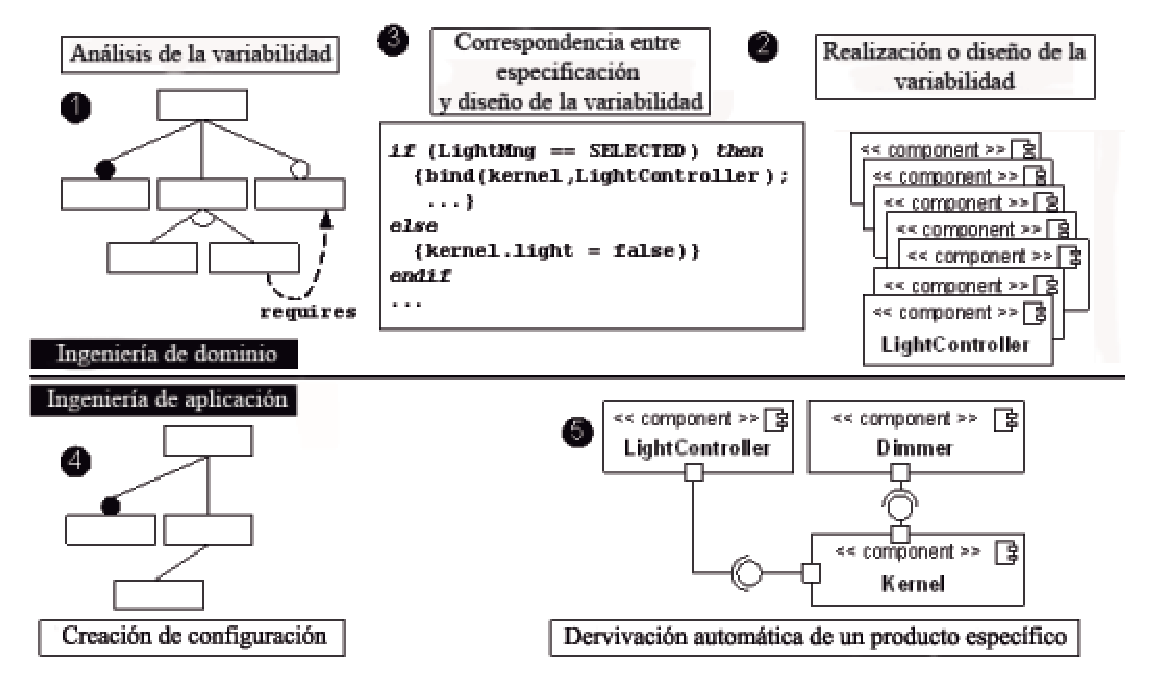
\includegraphics[width=.95\linewidth]{background/domainAplicationEngineering.eps} \\
  \caption{Proceso de desarrollo de una l�nea de productos software}
  \label{back:fig:domainAplicEng}
\end{figure}

En la fase de ingenier�a del dominio, el primer paso a realizar ser�a un an�lisis de qu� caracter�sticas de la familia de productos son variables y por qu� y c�mo son variables. Esta parte es la que se conoce como \emph{an�lisis o especificaci�n de la variabilidad} (Figura~\ref{back:fig:domainAplicEng}, punto 1). A continuaci�n, se ha de dise�ar una arquitectura o marco de trabajo para la familia de productos software que permita soportar dichas variaciones. Esta actividad se conoce como \emph{realizaci�n o dise�o de la variabilidad} (Figura~\ref{back:fig:domainAplicEng}, punto 2). El siguiente paso es establecer una serie de reglas que especifiquen como hay que instanciar la arquitectura previamente creada de acuerdo con las caracter�sticas seleccionadas por cada cliente. Esta fase es la que se conoce como \emph{correspondencia entre especificaci�n y dise�o de la variabilidad} (Figura~\ref{back:fig:domainAplicEng}, punto 3).

En la fase de ingenier�a de aplicaci�n, se crear�a una \emph{configuraci�n}, que no es m�s que una selecci�n de caracter�sticas que un usuario desea incluir en su producto (Figura~\ref{back:fig:domainAplicEng}, punto 4). En el caso ideal, usando esta configuraci�n, deber�amos poder ejecutar las reglas de correspondencia entre especificaci�n y dise�o de la variabilidad para que la arquitectura creada en la fase de ingenier�a del dominio se adaptase autom�ticamente generando un producto concreto espec�fico acorde a las necesidades concretas del usuario (Figura~\ref{back:fig:domainAplicEng}, punto 5). En caso no ideal, dichas reglas de correspondencia deber�n ejecutarse a mano, lo cual suele ser un proceso tedioso, largo, repetitivo y propenso a errores.

Este proyecto se centra en la primera etapa de este proceso de desarrollo, es decir en el an�lisis de la variabilidad de una familia de productos software mediante �rboles de caracter�sticas. La siguiente secci�n proporciona una breve pero completa descripci�n acerca del funcionamiento de los �rboles de caracter�sticas.


\section{�rboles de caracter�sticas}
\label{sec:back:fmodels}
%%==================================================================%%
%% Author : Tejedo Gonz�lez, Daniel                                 %%
%%          S�nchez Barreiro, Pablo                                 %%
%% Version: 1.0, 18/11/2012                                         %%                   
%% Version: 2.0, 05/02/2013                                         %%                   
%%                                                                  %%
%% Memoria del Proyecto Fin de Carrera                              %%
%% Antecedentes, �rboles de caracter�sticas                         %%
%%==================================================================%%

Como se ha comentado en la secci�n anterior, una de las tareas clave para el �xito de una l�nea de productos software consiste en analizar la variabilidad existente en la familia de productos software que dicha l�nea de productos software pretende cubrir. Aqu� es donde entran en juego los \emph{�rboles de caracter�sticas}~\cite{kang:1990, czarnecky:2005, danilo:2003}. Una \emph{caracter�stica} se define como ``\emph{un incremento en la funcionalidad del producto}'', o m�s formalmente, ``\emph{una caracter�stica es una propiedad de un sistema que es relevante a algunos \emph{stakeholders} y que es utilizada para capturar propiedades comunes o diferenciar entre sistemas de una misma familia}''~\cite{eisenecker:2000}. De este modo un producto queda representado por las caracter�sticas que posee.

Para poder capturar las divergencias y aspectos comunes entre los distintos productos de una misma familia, los �rboles de caracter�sticas organizan de forma jer�rquica el conjunto de caracter�sticas que posee una familia de productos. Cada caracter�stica se representa como un nodo en el �rbol de caracter�sticas. La ra�z de dicho �rbol es siempre el sistema o producto software cuya variabilidad estamos analizando. Cada caracter�stica se puede descomponer en varias subcaracter�sticas, siendo est�s �ltimas nodos \emph{hijos} de la primera caracter�stica, que actuar�a como \emph{padre}. Dependiendo de si dichas subcaracter�sticas son obligatorias, alternativas u opcionales, existen diversos tipos de relaciones padre-hijo. 

%%=========================================================================================%%
%% NOTA(Pablo): Para esta figura, hazte un modelo para la Smart Home sin habitaciones ni   %%
%%              plantas. Lo puedes encontrar en un art�culo que te mando luego             %% %%=========================================================================================%%
\begin{figure}[!tb]
    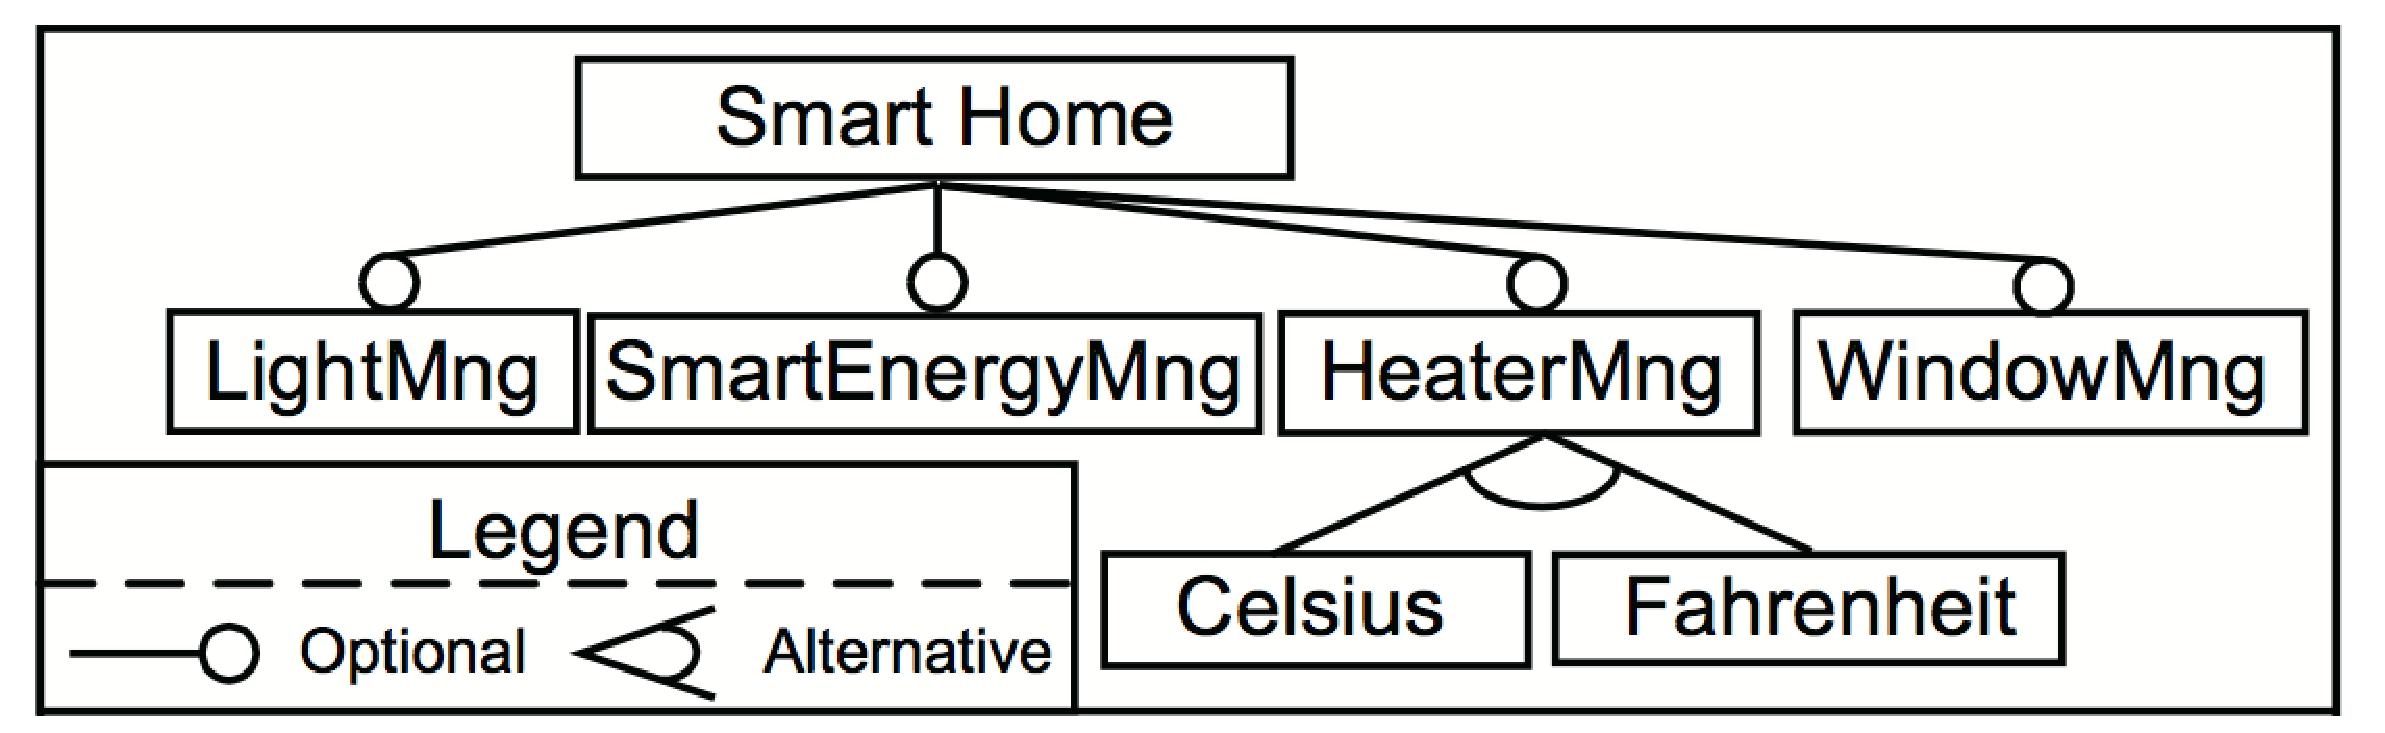
\includegraphics[scale=0.3]{background/simpleSmarthome.eps}
    \caption{�rbol de caracter�sticas simple para nuestro caso de estudio}
    \label{fig:smartHomeFMsimple}
\end{figure}

La Figura~\ref{fig:smartHomeFMsimple} muestra como ejemplo un �rbol de caracter�sticas que especifica la variabilidad inherente a nuestro caso de estudio, sin considerar que las plantas y habitaciones puedan configurarse de manera individual. El �rbol representa un hogar inteligente definido por las siguientes caracter�sticas: controlador de luz, controlador de temperatura, controlador de ventanas y controlador de la energ�a. Tal como se puede ver en la leyenda de la figura, todas estas caracter�sticas son opcionales, es decir, podemos decidir si queremos que est�n o no presentes en el hogar inteligente que generemos. Adem�s, para la caracter�stica ''controlador de temperatura" se ha de especificar una de las dos opciones alternativas que se plantean: grados celsius o grados fahrenheit.

El modo de representaci�n de los �rboles de caracter�sticas permite especificar cierto tipo de restricciones que pueden resultar necesarias para representar con exactitud el comportamiento del producto que queramos construir. En el caso de la Figura~\ref{fig:smartHomeFMsimple} se puede observar que mediante las relaciones ya se est� modelando la restricci�n que especifica que el controlador de temperatura ha de ser necesariamente de uno de los tipos que se indican en el modelo. Otros tipos de relaciones que pueden incluirse sirven para especificar otras restricciones, por ejemplo la obligatoriedad de seleccionar una caracter�stica o un grupo de ellas.

Sin embargo, si quisi�ramos incluir algunas restricciones m�s complejas, la representaci�n gr�fica de los �rboles de caracter�sticas se queda corta. Por ejemplo, en la Figura~\ref{fig:smartHomeFMsimple} podr�amos querer especificar la restricci�n de que si nuestro hogar inteligente tiene un controlador de energ�a, ha de tener tambi�n un controlador de calefacci�n en grados celsius. Es imposible modelar esta restricci�n con las herramientas de las que los �rboles de caracter�sticas disponen. Es por ese motivo que debe permitirse la posibilidad de especificar restricciones externas al �rbol mediante alg�n tipo de lenguaje textual o gr�fico.

%%=========================================================================================%%
%% NOTA(Pablo): Explicar el modelo creado, indicando las cosas que son variables, las que  %%
%%              son alternativas, etc.                                                     %%
%%              Explicar el problema de las restricciones externas                         %%
%%=========================================================================================%%

\begin{figure}[!tb]
    \centerline{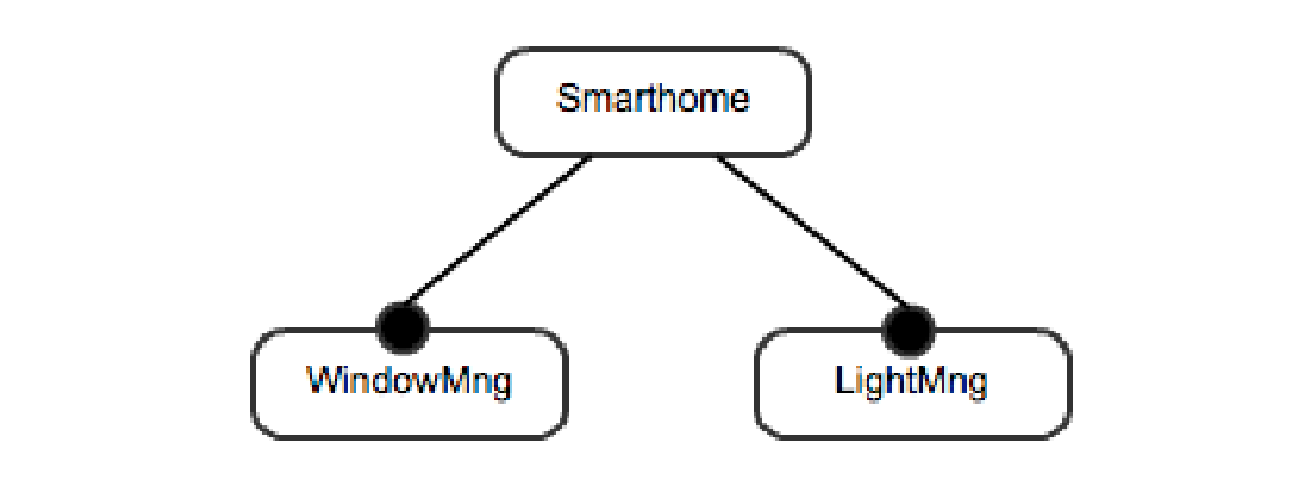
\includegraphics[scale=0.3]{background/simpleSmarthomeConf.eps}}
    \caption{Configuraci�n para la versi�n sencilla del caso de estudio}
    \label{fig:smartHomeConfSimple}
\end{figure}

Una vez creado un �rbol de caracter�sticas para una l�nea de productos software, podemos indicar las caracter�sticas que podemos incluir en un producto software concreto mediante la creaci�n de configuraciones. Una \emph{configuraci�n} no es m�s que una selecci�n v�lida de caracter�sticas. La Figura~\ref{fig:smartHomeConfSimple} muestra en un ejemplo de configuraci�n para el modelo de la Figura~\ref{fig:smartHomeFMsimple} donde se indica que el producto que deseamos construir debe incluir �nica y obligatoriamente un dispositivo de control de luz y un dispositivo de control de ventanas. Obviamente, dicho modelo debe satisfacer las restricciones externas declaradas. 

Los �rboles de caracter�sticas como los anteriormente expuestos no permiten modelar que pueda existir un n�mero variable de ciertas caracter�sticas, como, en nuestro caso, de plantas y habitaciones, y que, adem�s, cada instancia particular de una caracter�sticas pueda  configurarse de forma distinta. Por ejemplo, podr�amos decidir que el sal�n de la casa tenga control inteligente de temperatura, mientras que la cocina, que est� sometida a mayores variaciones de temperatura, no contenga dicha caracter�sticas. Para solventar esta carencia, se introdujeron en los �rboles de caracter�sticas el concepto de caracter�stica clonable. 

\begin{figure}[!tb]
    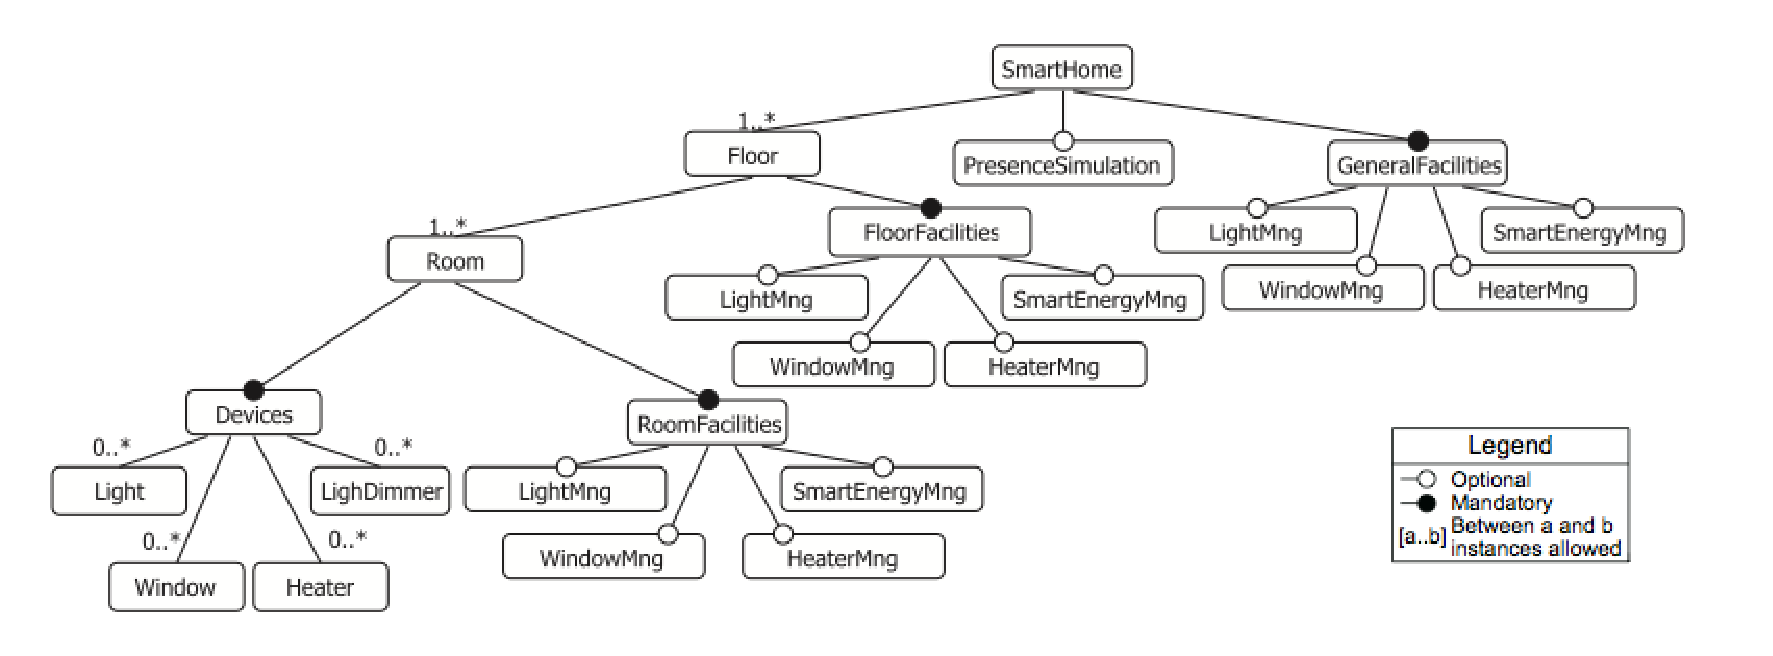
\includegraphics[scale=0.4]{background/featuremodel.eps}
    \caption{�rbol de caracter�sticas completo para nuestro caso de estudio}
    \label{fig:smarHomeFeatureModel}
\end{figure}

La Figura~\ref{fig:smarHomeFeatureModel} muestra el �rbol de caracter�sticas para nuestro caso de estudio incluyendo \emph{caracter�sticas clonables}. Las caracter�sticas \emph{Floor} (Piso) y \emph{Room} (Habitaci�n) son clonables porque pueden aparecer m�s de una vez en las configuraciones creadas. La cardinalidad de ambas caracter�sticas es 1..*, lo que significa que pueden ser seleccionadas de una a infinitas veces. As� mismo, cualquier caracter�stica que sea hija de ellas directa o indirectamente es considerada inmediatamente como caracter�stica. Este es el caso, por ejemplo, de \emph{Devices} y de sus caracter�sticas hijas (\emph{Heater}, \emph{Window}, etc.), que son consideradas clonables tanto por su cardinalidad como por ser hijas de una caracter�stica clonable. 

La repetici�n de las caracter�sticas correspondientes a los diversos controladores (es decir, \emph{WindowMng}, \emph{HeaterMng}, etc.) se debe a que gracias a las caracter�sticas clonables ahora podemos diferenciar los controladores seg�n su colocaci�n y alcance. Es decir, el controlador de temperatura hijo de \emph{RoomFacilities} afectar� s�lo a la habitaci�n a la que pertenezca, el hijo de \emph{FloorFacilities} afectar� al piso al que pertenezca, y el hijo de \emph{GeneralFacilities} afectar� a todo el hogar creado. 
%%=========================================================================================%%
%% NOTA(Pablo): A�adir la figura, si no te entrase bien a lo ancho, mira como meterla 
%%              apaisada en Latex.
%%=========================================================================================%%

A la hora de crear configuraciones para este nuevo �rbol hay que tener en cuenta que podemos seleccionar en m�s de una ocasi�n ciertas caracter�sticas, por lo que necesitamos valernos de alg�n mecanismo que nos permita diferenciarlas entre ellas. El modo de lograrlo es poniendo un nombre a las diferentes selecciones o clones que hagamos de una misma caracter�stica. 

La Figura~\ref{fig:smarthomeCompleteConf} muestra un ejemplo de configuraci�n para el �rbol de caracter�sticas con caracter�sticas clonables de la Figura~\ref{fig:smarHomeFeatureModel}. En ella se puede apreciar que se diferencia entre las diferentes selecciones de la caracter�stica \emph{Floor} poni�ndoles un nombre, en este caso \emph{Ground} (Planta Baja) y \emph{First} (Primer Piso). Del mismo modo con las habitaciones \emph{Kitchen} (Cocina) y \emph{Living} (Sal�n), pertenecientes a la planta baja, y \emph{Bed} (Dormitorio), perteneciente al primer piso. Observando el �rbol de la figura es sencillo comprender qu� elementos y/o controladores tiene instalados cada estancia. Por ejemplo, la cocina est� dotada de dos luces, un regulador de luz, una ventana, un controlador de luz y un controlador de ventanas.

%%=========================================================================================%%
%% NOTA(Pablo): Explicar como se configuran las caracter�sticas clonables usando un 
%%              ejemplo
%%=========================================================================================%%

Como en el caso anterior, las diversas configuraciones no s�lo han de cumplir las restricciones impuestas por el propio �rbol de caracter�sticas, sino tambi�n las restricciones externas. Pero debido a la presencia de caracter�sticas clonables ahora existe un abanico mucho mayor de restricciones posibles que definir. Del mismo modo que antes se pod�an definir diversas restricciones l�gicas ($a implies b$), la presencia de caracter�sticas clonables hace que tambi�n sean necesarias las restricciones num�ricas ($a >= b$), lo que tambi�n a�ade la dificultad de diferenciar qu� caracter�sticas pueden realizar operaciones l�gicas y cuales no. 

Tambi�n es necesaria una operaci�n de contexto que permita aplicar estas restricciones s�lamente a sub�rboles de la configuraci�n. Esto es imprescindible para definir una restricci�n que, por ejemplo, valide que si una habitaci�n tiene un controlador de ventanas, forzosamente ha de tener instalada al menos una ventana. Sin la operaci�n de contexto ser�a imposible saber a qu� caracter�stica \emph{WindowMng} en concreto est� haciendo referencia la restricci�n definida.

El objetivo de este proyecto es implementar un lenguaje textual que haga posible la definici�n de restricciones externas para �rboles de caracter�sticas con caracter�sticas clonables con todas las peculiaridades definidas anteriormente, as� como una herramienta que permita validar si las configuraciones creadas satisfacen o no esas restricciones. 
%%=========================================================================================%%
%% NOTA(Pablo): Explicar el problema de las restricciones cuando incluyen caracter�sticas
%%              clonables y decir que implementar un lenguaje para resolver ese problema 
%%              es el objetivo de este proyecto
%%=========================================================================================%%

%%=========================================================================================%%
%% NOTA(Pablo): Esto no se entiende de forma clara, por lo que se suprime                                         %%
%%=========================================================================================%%
%%
%% Por otro lado, un modelo de caracter�sticas debe poder representar la cardinalidad de 
%% las caracter�sticas, por motivos tanto de comprensi�n (es mucho mejor contar con un 
%% �rbol de 8 nodos que con uno de 100, teniendo ambos un significado equivalente), como 
%% de funcionalidad, ya que permite expresar ciertas restricciones que de no contar con 
%% la cardinalidad no podr�an expresarse.
%% 
%% Adem�s se podr�n disponer de restricciones de usuario m�s complejas, que son las que
%% se han implementado en el editor de especificaci�n y validaci�n de restricciones 
%% desarrollado en este proyecto.
%%
%%=========================================================================================%%

%%=========================================================================================%%
%% NOTA(Pablo): Esto queda obsoleto en el nuevo esquema, por lo cual se suprime            %%
%%=========================================================================================%%
%%
%% La figura \ref{fig7} muestra un ejemplo de modelo de caracter�sticas. En este caso se 
%% trata de un modelo de una casa inteligente o SmartHome, a trav�s del cual, 
%% seleccionando ciertas caracter�sticas u otras podremos construir qu� tipo de casa 
%% queremos. Cada una de las m�ltiples casas diferentes que podamos construir es lo que 
%% se denonima una especializaci�n o configuraci�n de nuestro modelo de caracter�sticas.
%% 
%%  El proceso de crear una configuraci�n a partir de un modelo de caracter�sticas se 
%% conoce como proceso de configuraci�n o proceso de especializaci�n. Consiste en 
%% transformar un modelo de caracter�sticas de tal forma que el modelo resultante sea un
%%  subconjunto de las posibles configuraciones denotadas por el primer modelo. La figura 
%% \ref{fig8} muestra una posible configuraci�n para el modelo de caracter�sticas de la figura %% \ref{fig7}.
%%
%% La relaci�n entre un diagrama de caracter�sticas y una configuraci�n es an�loga a la
%% existenteentre una clase y una de sus instancias en programaci�n orientada a objetos.
%%
%%=========================================================================================%%

\begin{figure}[!tb]
    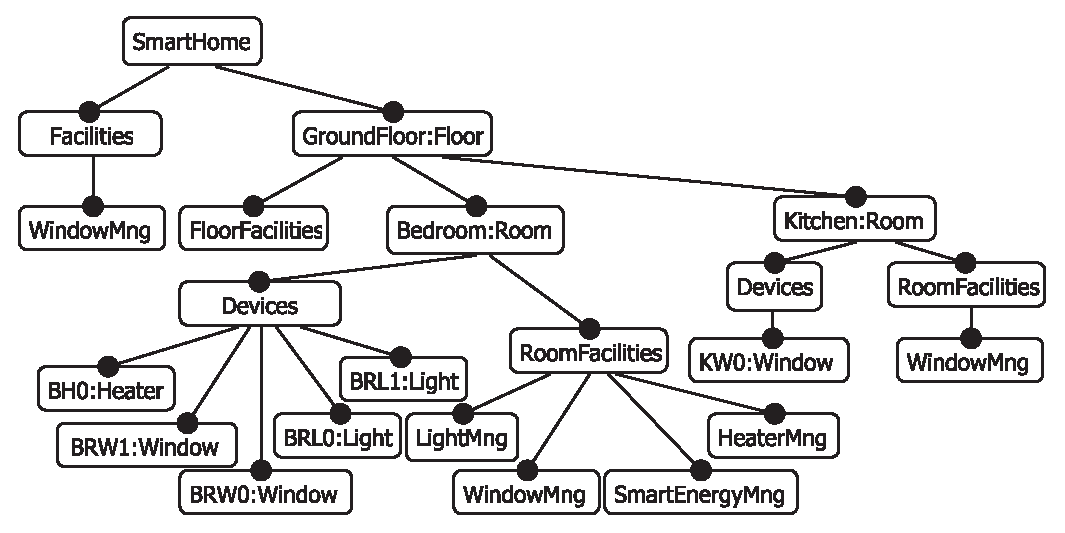
\includegraphics[scale=0.4]{background/configuration.eps}
    \caption{Posible modelo de configuraci�n de una casa inteligente concreta}
    \label{fig:smarthomeCompleteConf}
\end{figure}

\begin{figure}[!tb]
    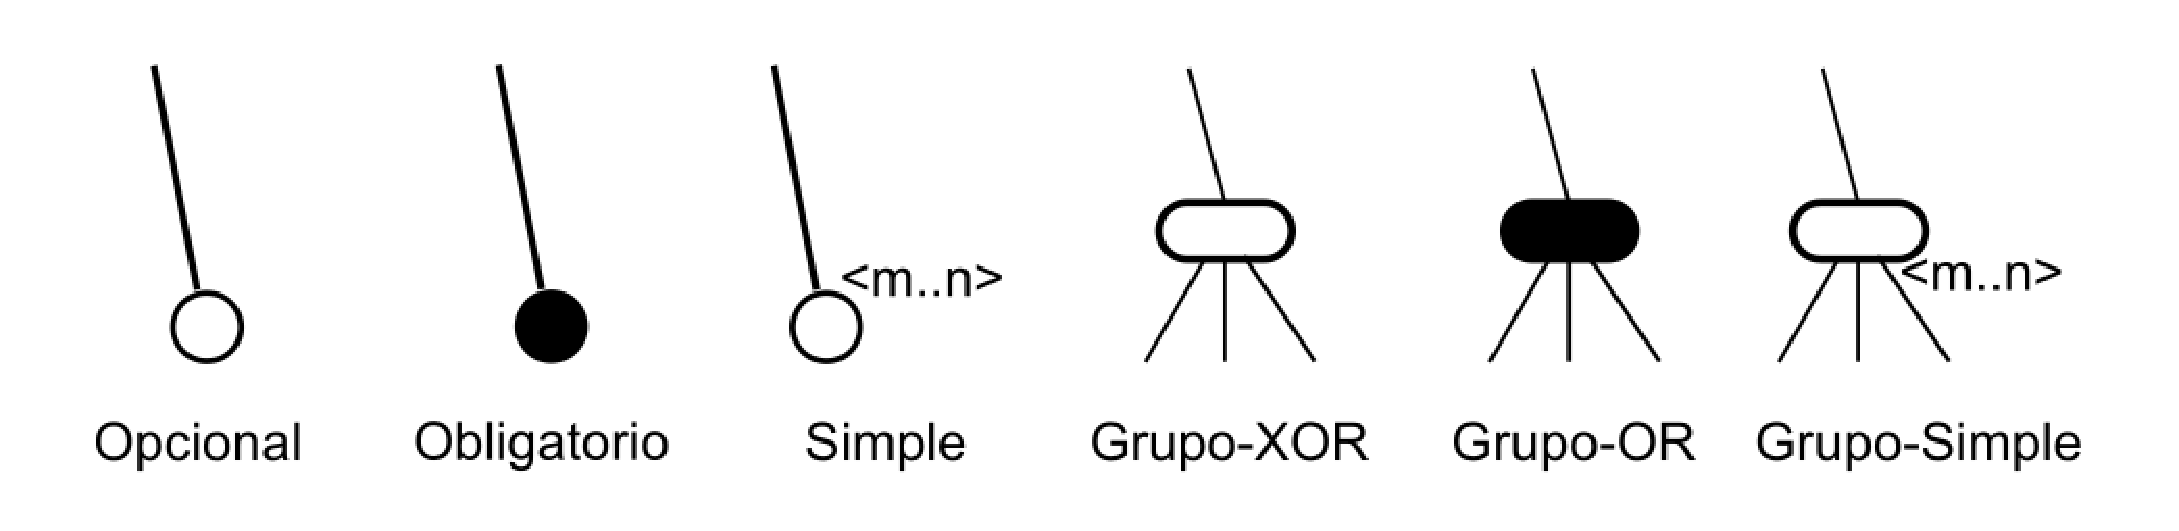
\includegraphics[scale=0.35]{background/relations.eps}
    \caption{Tipos de relaciones entre caracter�sticas }
    \label{fig:relacionesFeatures}
\end{figure}

A modo de resumen, la Figura~\ref{fig:relacionesFeatures} muestra las posibles relaciones que pueden entre caracter�sticas, as� como su representaci�n gr�fica. Dichas relaciones se describen a continuaci�n:

\begin{description}
    \item[Opcional] La caracter�stica hija puede estar o no estar seleccionada
    \item[Obligatoria] La caracter�stica siempre debe estar seleccionada.
    \item[Clonable] La caracter�stica tendr� una cardinalidad $<m,n>$, siendo m y n n�meros enteros que denotan el m�nimo y el m�ximo respectivamente de caracter�sticas que podemos seleccionar.
    \item[Grupo-xor] S�lo una de las caracter�sticas pertenecientes al grupo puede ser seleccionada.
    \item[Grupo-or] Debemos seleccionar como m�nimo una de las subcaracter�sticas, pudiendo seleccionar m�s si lo deseamos.
    \item[Grupo con cardinalidad] El n�mero m�nimo y m�ximo de caracter�sticas a seleccionar dentro del grupo vendr� determinado por su cardinalidad $<m,n>$.
\end{description}

Tras esta secci�n se han proporcionado al lector lo necesario para comprender el contexto del problema que este Proyecto Fin de Carrera pretende resolver. Las siguientes secciones est�n destinadas a explicar las tecnolog�as concretas que se han utilizado para implementar el lenguaje que da soluci�n a los problemas planteados. 


\section{\emph{Eclipse Modelling Framework}}
\label{sec:back:ecore}
%%==================================================================%%
%% Author : Tejedo Gonz�lez, Daniel                                 %%
%%          S�nchez Barreiro, Pablo                                 %%
%% Version: 1.0, 18/11/2012                                         %%                  
%%                                                                  %%
%% Memoria del Proyecto Fin de Carrera                              %%
%% Antecedentes, ecore                                              %%
%%==================================================================%%

EMF \emph{Eclipse Modeling Framework}~\cite{} es un \emph{plug-in} para Eclipse~\cite{} que permite elaborar metamodelos. Pera ello proporciona un lenguaje de metamodelo denominado Ecore, el cual se ha convertido en el est�ndar de factor para la realizaci�n de metamodelos. Utilizando Ecore se pueden crear metamodelos de forma gr�fica usando una notaci�n muy similar a la los diagramas de clases de UML. La Figura~\ref{fig:sle:metamodeloGrafo} muestra un sencillo ejemplo de metamodelo en Ecore (ver Secci�n~\ref{sec:intr:sle} para m�s detalles). EMF tambi�n incorpora una herramienta para la validaci�n reglas adicionales que no puedan ser especificadas a nivel de del metamodelo. 
 
EMF permite que, a partir de un metamodelo especificado en Ecore, podamos, utilizando diversos generadores de c�digo, crear autom�ticamente un conjunto de clases que nos permiten manipular dichos modelos a nivel de c�digo. Dichas clases se pueden adem�s distribuir como \emph{plug-in} para el entorno Eclipse.

Adem�s, al haberse convertido en est�ndar \emph{de facto} para el desarrollo de metamodelos, Ecore es compatible con multitud de herramientas para Ingenier�a de Lenguajes Dirigida por Modelos, como EMFText, la cual se describe en la siguiente secci�n, o diversos generadores de c�digo o herramientas de transformaci�n de modelos. 



\section{EMFText}
\label{sec:back:emftext}
%%==================================================================%%
%% Author : Tejedo Gonz�lez, Daniel                                 %%
%%          S�nchez Barreiro, Pablo                                 %%
%% Version: 1.0, 18/11/2012                                         %%                   %%                                                                  %%
%% Memoria del Proyecto Fin de Carrera                              %%
%% Antecedentes, emftext                                      %%
%%==================================================================%%


EMFText es una herramienta espec�ficamente dise�ada para dise�ar las gram�ticas de los lenguajes que hayan sido dise�ados previamente con un metamodelo de Ecore. Est� especializado para la creaci�n de Lenguajes Espec�ficos de Dominio, aunque tambi�n se pueden crear lenguajes de prop�sito general. 

Pero, como en casi todos los casos de este tipo de herramientas, su mayor virtud es la enorme cantidad de c�digo autogenerado que produce, y que elimina al programador de tareas tediosas que adem�s en muchos casos podr�an resultar complicadas. Todo el c�digo generado es completamente independiente de EMFText, es decir, podr� ser ejecutado en plataformas que no tengan la herramienta instalada. 

Todo el c�digo generado por EMFText est� dise�ado de tal modo que sea f�cil de modificar en caso de que queramos poner en pr�ctica algunas funcionalidades poco habituales. Se facilita mucho la labor a la hora de modificar estructuras como el postprocesador de nuestra gram�tica. Todas las gram�ticas construidas tendr�n que ser LL por defecto, a no ser que queramos modificar los parsers generados, posibilidad tambi�n disponible. 

Otro tipo de funcionalidades implementadas, quiz�s no tan importantes pero tambi�n de gran utilidad, son el coloreado de c�digo (por defecto o personalizable), funci�n de completar c�digo, generaci�n del �rbol parseado en el la vista de eclipse Outline o generaci�n de c�digo para crear un depurador para nuestro lenguaje.

\begin{figure}[t]
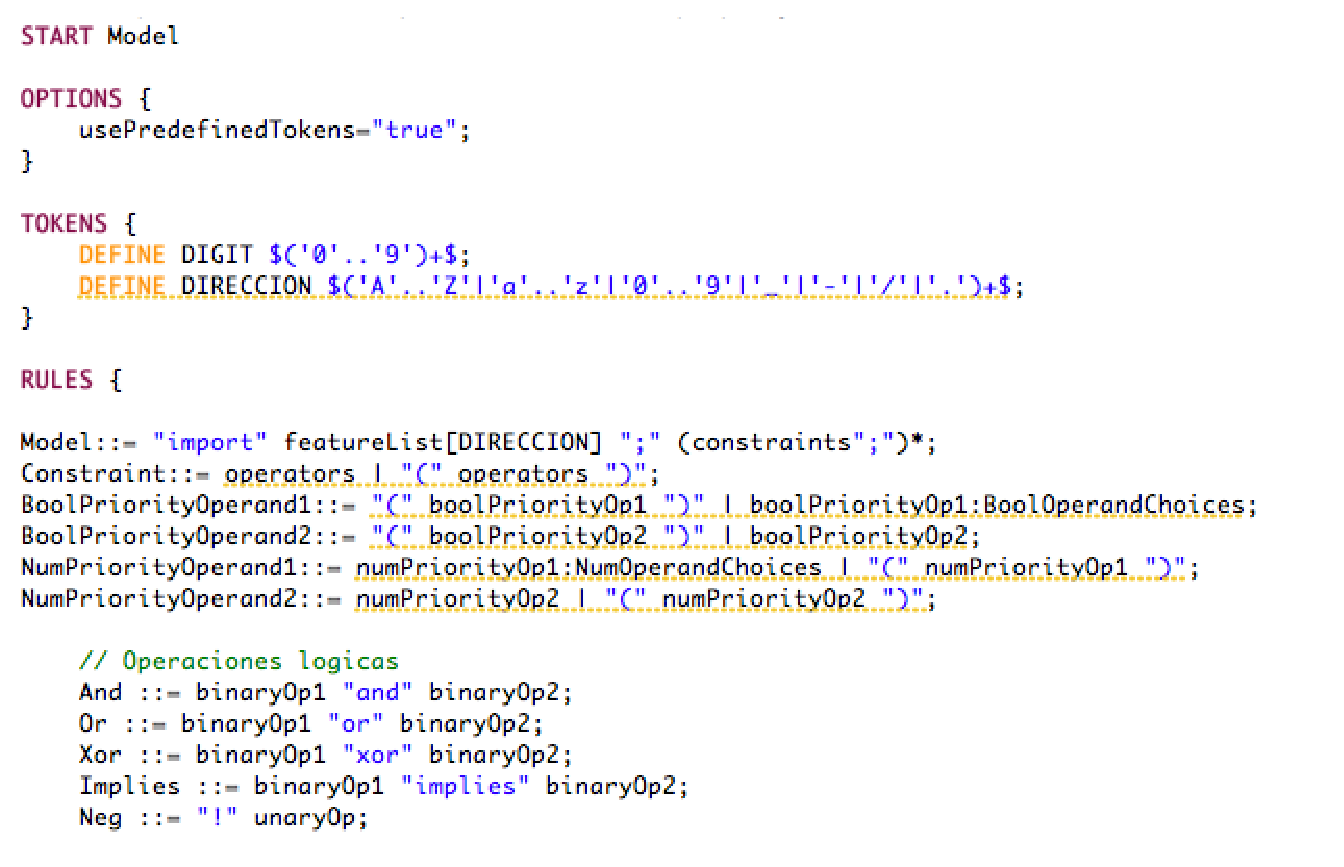
\includegraphics[scale=0.5]{background/gramatica.eps}
\caption{Trozo de la gram�tica de nuestro editor de especificaci�n y validaci�n de restricciones}
\label{fig5}
\end{figure}


EMFText permite la definici�n de gram�ticas utilizando un lenguaje est�ndar para la definici�n de expresiones regulares, adem�s de incorporar algunas particularidades propias que facilitan ciertas tareas. En la figura \ref{fig5} se muestra una peque�a captura que contiene una porci�n de la gram�tica construida para nuestro editor de especificaci�n y validaci�n de restricciones. 

\section{Arquitectura de plugins de Eclipse}
\label{sec:back:eplugins}
%%==================================================================%%
%% Author : Tejedo Gonz�lez, Daniel                                 %%
%%          S�nchez Barreiro, Pablo                                 %%
%% Version: 1.0, 18/11/2012                                         %%                   
%% Version: 1.0, 06/02/2013                                         %%                   
%%                                                                  %%
%% Memoria del Proyecto Fin de Carrera                              %%
%% Antecedentes, arquitectura de plugins de eclipse                 %%
%%==================================================================%%

El entorno de desarrollo Eclipse es un ejemplo de arquitectura modular f�cilmente extensible mediante una compleja, pero sencilla para el programador, arquitectura de \emph{plug-ins}. Un \emph{plug-in} en Eclipse es un componente que provee un cierto tipo de servicio dentro del contexto del espacio de trabajo de Eclipse. Es decir, una herramienta que se puede integrar en el entorno Eclipse junto con sus otras funcionalidades. Dado que la herramienta \emph{Hydra} fue dise�ada como un \emph{plug-in} para Eclipse, y nuestro editor pretende integrarse tanto en \emph{Hydra} como en \emph{Eclipse}, es necesario conocer y manejar el funcionamiento de la arquitectura de plug-ins de Eclipse.

Aunque la arquitectura de plug-ins de Eclipse tiene mucha profundidad y ofrece muchas posibilidades, es imprescindible el dominio de dos de sus conceptos clave para poder trabajar con ella: las dependencias y los puntos de extensi�n. Mediante las dependencias podemos indicar que el plug-in a desarrollar tiene que incorporar toda la funcionalidad y estructura de otro plug-in (en este caso nuestro editor tiene, entre otras, una dependencia con el plug-in de la herramienta Hydra original). Un punto de extensi�n permite a�adir cierta funcionalidad al plug-in desarrollado mediante la inclusi�n autom�tica de ciertos segmentos de c�digo. Un ejemplo cl�sico de punto de extensi�n, y que adem�s ha sido utilizado en el transcurso de este proyecto, es el que permite a�adir un bot�n a la barra de tareas de Eclipse de manera autom�tica, teniendo que implementar �nicamente el c�digo del manejador de ese bot�n.

 \begin{figure}[!tb]
    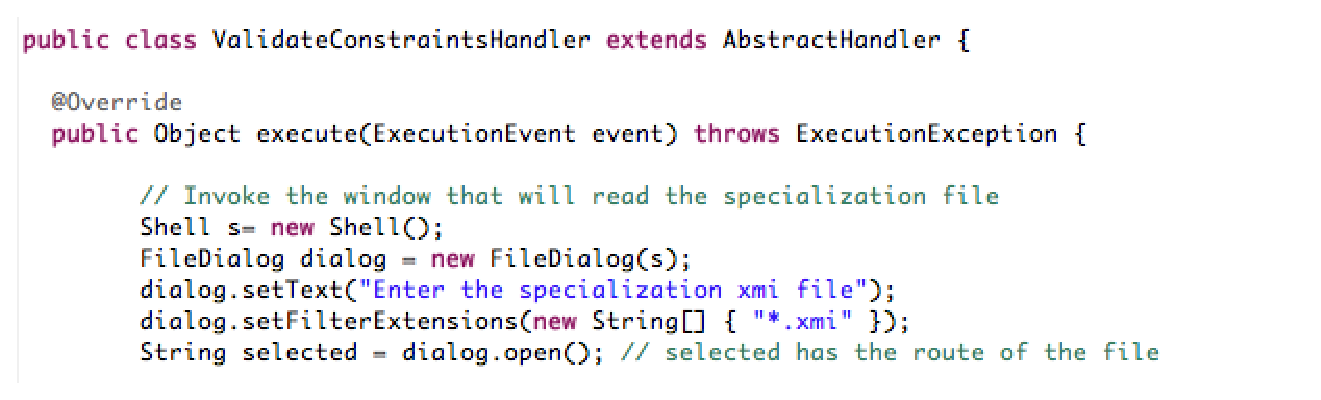
\includegraphics[scale=0.4]{background/codigoManejador.eps}
    \caption{Trozo de c�digo del manejador de un bot�n introducido mediante un punto de extensi�n}
    \label{fig:codigoManejador}
\end{figure}

%%==============================================================================================%%
%% NOTA(Pablo): Esto no se entiende nada
%%==============================================================================================%%
%%
%% En particular, se han utilizado mucho los puntos de extensi�n. Un punto de extensi�n en un
%% plug-in indica la posibilidad de que ese plug-in sea a su vez parte de otro, o que haya 
%% otros plug-ins que sean parte de �l. Esta particularidad permite no s�lo la integraci�n de 
%% nuestro editor con Hydra, sino tambi�n la personalizaci�n de men�s y botones para �l 
%% gracias a la creaci�n de puntos de extensi�n con plug-ins de creaci�n de men�s y barras de
%% herramientas.
%%
%%==============================================================================================%%

%%==============================================================================================%%
%% NOTA(Pablo): Para solucionar
%% - Describir en uno o dos p�rrafos c�mo funciona la arquietctura de plug-ins para Eclipse
%% - Poner un ejemplo de punto de extensi�n, sencillo y concreto, y explicar como funciona 
%%   el punto de extensi�n utilizando algo de c�digo.
%% Si no sabes como escribir esta secci�n, la eliminas directamente, y actualizas la intro 
%% al Cap�tulo de forma conveniente.
%%==============================================================================================%%


\section{Sumario}
\label{sec:back:sumario}
%%==================================================================%%
%% Author : Tejedo Gonz�lez, Daniel                                 %%
%%          S�nchez Barreiro, Pablo                                 %%
%% Version: 1.0, 25/11/2012                                         %%                   
%%                                                                  %%
%% Memoria del Proyecto Fin de Carrera                              %%
%% Sintaxis abstracta, sumario                          %%
%%==================================================================%%

Durante el presente cap�tulo se ha descrito el proceso de definici�n de la sintaxis abstracta de nuestro lenguaje. Este proceso abarca subtareas como la captura de requisitos del lenguaje, la creaci�n de un metamodelo que permita la creaci�n de sintaxis concretas apropiadas, la validaci�n de restricciones externas a ese metamodelo, y las pruebas que corroboren que todos los elementos creados funcionan correctamente. En el siguiente cap�tulo profundizaremos acerca del dise�o de la gram�tica para nuestro lenguaje, as� como de las herramientas utilizadas para implementar esa gram�tica.


\subsection{New research challenges on clonable features}

The creation of clonable features was initially an easy task, since it only required to add the notion of cardinality to each feature. Nevertheless, this has created several side-effects, since some concepts such as the semantics of a clonable feature selection, had to be reviewed and updated. This section identifies several problems, not currently solved to the best of our knowledge, regarding the specification of external constraints involving clonable features.

Let us explain our motivating scenario. In Figure~\ref{fig:smartHomeFM}, house facilities can be selected at a house, floor or room level. Obviously, if we select the \imp{SmartEnergyMng} feature, this implies that the \imp{LightMng} and the \imp{HeaterMng} must also be selected. This need to be specified as a external constraint. There are also some other constraints between features, such as, for instance, if \imp{LightMng} is selected at the floor level, this facility must also be selected for each room contained in such a floor. 

% Nevertheless, this had several consequences, since it was required to review an update well-established concepts related 
% to feature modelling and to answer several research challenges that emerged as a consequence of introducing this new 
% concept. Previous section described how clonable features are selected by means of a new cloning operation. This section 
% identifies several problems, not currently solved to the best of our knowledge, regarding the specification of external 
% constraints between features when some of the features involved in the constraint are clonable.

When dealing with feature models without clonable features, the most usual way to express these external constraints is by means of propositional formulas, like \imp{SmartEnergyMng implies (LightMng and HeaterMng)}, where the features are the atoms for these formulas~\cite{batory:2005}. A feature is true when the feature is selected, and false when unselected. The main problem when dealing with clonable features is that this correspondence is not true anymore, since clonable features are not simply selected or unselected, they are cloned. So, the semantics of these logical expressions become undefined.

For instance, let us suppose  \imp{A} and \imp{B} are clonable features. In this case, what would be the semantics of a external constraint like \imp{A implies B}? Does this means that one instance of \imp{A} implies the existence of at least one instance of \imp{B}? Or, otherwise, does it means that the existence of all potential \imp{A}s implies the existence of all potential \imp{B}s? So, the first research challenge we face is to decide what a clonable feature means in a logical formula.

% Or maybe all potential \imp{A}s only implies the existence of one \imp{B}?

Since clonable features has asscoiated a set of clones, we might want to specify properties that only applies to: (1) at least one element of the set; (2) to all the elements of the set that fulfill a certain constraint; or (3) all the elements. For instance, we might want to specify constraint such as: if \imp{HeaterMng} is selected per house level, at least one \imp{Room} must contain a \imp{Heater}. So, the second research challenge is to add quantification mechanisms to constraints involving clonable features.

Moreover, we might want to specify constraints which must be evaluated for a particular subtree of the whole feature model, i.e. in a particular \emph{context}. For instance, if \imp{LightMng} has been selected as facility for a particular \imp{Room}, such a \imp{Room} must have at least one clone of \imp{Light}. If we specify a constraint ``\imp{LightMng} implies at least one \imp{Light}'', but we do not limit the scope in which this constraint is evaluated, this constraint might be true for the configurations of Figure~\ref{fig:contexts} (a) and (b). Nevertheless, this constraint should be false for Figure~\ref{fig:contexts} (a), since \imp{r1:Room} has selected the \imp{LightMng} facility, but it has not \imp{Light} to control. This means this constraint must be evaluated for all rooms (notice we need again quantification) and using only the subtree below each \imp{Room}. Thus, the third research challenge is to specify the context where each constraint must be evaluated. 

% Figure~\ref{fig:contexts} contains an example and a counterexample for this situation. 

% i.e. we use the whole feature model for evaluating the constraint, this constraint will be true for the configuration of 
% Figure~\ref{fig:contexts} (a) and (b). Nevertheless, this constraint should be not satisfied by the configuration of 
% Figure~\ref{fig:contexts} (a) is not correct, since \imp{r1:Room} has selected the \imp{LightMng} facility, but it has 
% not \imp{Light} to control. 

% Contexts are also useful for solve ambiguities when using feature references, since multiple copies of a same feature 
% might appear at different part of a configuration model. For instance, does \imp{LightMng} refers to \imp{LightMng} for 
% \imp{GeneralFacilities}, \imp{FloorFacilities} or \imp{RoomFacilities}. Using contexts, we can limit the scope of a name % to unambiguously refer to a certain feature. 

\begin{figure}
  % Requires \usepackage{graphicx}
  \centering 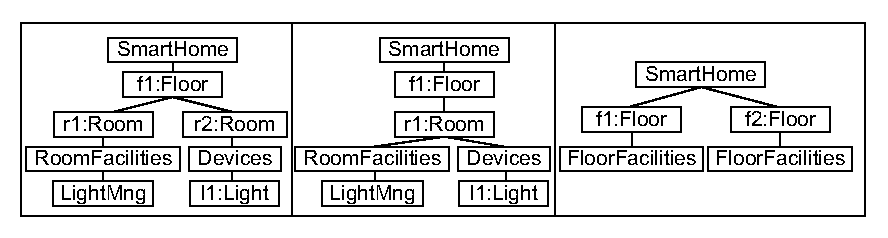
\includegraphics[width=.7\linewidth]{Figures/contexts(2).eps} \\
  \caption{(a) Invalid configuration (b) Valid configuration (c) Multiple features}
  \label{fig:contexts}
\end{figure}

Finally, when dealing with clonable feature, not only clonable features can appear more than one time in a configuration model. A feature can appear more than one time one of its ancestors is clonable. Figure~\ref{fig:contexts} (a) illustrates this situation. We call to a feature that can appear more than one time a \emph{multiple feature}. For instance, the feature \imp{FloorFacilities}, which is not clonable itself,  might appear several times in a configuration model as a consequence of the \imp{Floor} feature being cloned. This implies that \imp{FloorFacilities} also evaluates to a set of features when it is evaluated in the context of the entire configuration model. Nevertheless, it should be noticed that this feature can be evaluated to true or false if it is evaluated in the context of a \imp{Floor} feature, since it can appear only once in that context. So, a last research challenge is how to deal appropriately with \emph{multiple features}.

Summarising, when dealing with clonable features, we need to address the following research challenges in order to properly express constraints between features:

\begin{enumerate}
    \item What a clonable feature means inside a constraint expression.
    \item Add quantification mechanisms to constraints expressions.
    \item Add the notion of contexts to constraints expressions and subexpressions.
    \item Design a mechanism for properly dealing with clonable features.
\end{enumerate}

State-of-art tools only offer two operators, \imp{implies} and \imp{excludes}, and deal with simple propositional formulas. This is clearly not enough to address the research challenges described in this section.
To solve this limitation, we have created an expressive language for expressing arbitrary complex constraints in a user-friendly fashion and we have implemented a reasoner able to decide if a set of external constraints, involving
clonable or multiple features, is satisfied given a specific configuration of a feature model. The reasoner is also able to perform some extra task, such as deciding which features must be incorporated to a configuration in order to satisfy the external constraints. We have integrated this language and the reasoner in our feature modelling environment, which we have called \emph{Hydra}.

Next section describes the language for expressing external constraints involving clonable features and the reasoner that analyse the satisfiability of these constraints.

%\emph{Hydra}, a tool for modelling, configuring and validating cardinality-based features models, i.e. feature models
% that contain \emph{clonable features}. This has implied we have had to review the way in which clonable features are
% configured, and, overall, how user-defined constraints are defined and evaluated in the presence on clonable
% features.

%==================================================================================================%
% NOTE(Pablo): Out                                                                                 %
%==================================================================================================%

% A typical feature modelling process would be as follows:
%
% \begin{enumerate}
%    \item First of all, a feature model is created. A feature model is a tree representation of the features included in % a set of products and of the relationships between them.
%    \item Since not all the relationships between features can be captured using simply the syntax provided by feature
% models, it is often required to specify some external constraints, which restrict the way in which features in a
% feature model can be selected. For instance, we might specify that if a certain feature \imp{A} is selected, another
% feature \imp{B} can not be selected, due to a bad interaction between these features.
%    \item Once we have created a feature model, we can use it for creating configurations, i.e. selection of features
% that specify which particular features are, or it will be, included in a certain product.
%    \item To ensure we are creating correct configurations, we need to validate that a configuration obeys the rules the % syntax of the feature model, and, in addition, it also satisfies the external defined constraints.
% \end{enumerate}

% Feature models have experimented several evolutions in last decade. Recently, Czarnecki et al~\cite{czarnecki:2005}
% introduced the simple but powerful concept of \emph{clonable feature}. A clonable feature is a feature that can appear % with a variable number of instances in different products. For instance, when modelling automated houses, clonable
% features are \emph{rooms} and \emph{floors}, since automated houses can have a variable number of floors and rooms.
% The creation of clonable features was initially an easy tasks, since it only required to add a cardinality to each
% feature contained in the feature model.



%========================================================================%
% NOTA : Perhaps it is better to move this section at the end, mainly    %
%        because to explain why our tool improves the state-of-art, we   %
%        need to                                                         %
%========================================================================%

\section{Expressing and validating constraints involving clonable features}
\label{sec:theLanguage}

%============================================================================%
% Author: Pablo S�nchez                                                      %
%         p.sanchez@unican.es, http://personales.unican.es/sanchezbp         %
% Section : The language                                   Date: 28/02/2011  %
% Version : 1.0                                                              %
% Conference: SPLC 2011                                                      %
%============================================================================%

% \subsection{Expressing external constraints with clonable features}
% %===============================================================================%
% Author: Pablo S�nchez (pablo@lcc.uma.es; http://www.lcc.uma.es/~pablo)        %
% Section : Expressing...                                    Date: 02/12/2009   %
% Version : 1.0                                                                 %
% Conference: Caise 2010                                                        %
%===============================================================================%

%===============================================================================%
% NOTE(Pablo): Check with the work I did in Santander and with the work I did   %
%              at home                                                          %
%===============================================================================%

\begin{figure}
    \begin{scriptsize}
    \begin{verbatim}
00 <Constraint> ::= "true" | "false" | <SimpleFeature> | <Constraint> <BinaryOp> <Constraint> |
01                  <UnaryOp> <Constraint> | "(" <Constraint> ")" | <ContextExp> |
02                  <ComparisonExp>;
03 <BinaryOp>   ::= "and" | "or" | "xor" | "implies";
04 <UnaryOp>    ::= "not";
05 <ContextExp> ::= <SimpleFeature> "[" <Constraint> "]" |
06                  "all" <MultiValueFeature> "[" <Constraint> "]" |
07                  "any" <MultiValueFeature> "[" <Constraint> "]";
08 <ComparisonExp> ::= <NumericalExp> <ComparisonOp> <NumericalExp>;
09 <ComparisonOp>  ::= "<" | "<=" | "=" | "=>" | ">" | "!=";
10 <NumericalExp>  ::= <MultiValueFeature> | "PositiveInteger" |
11                     <MultiValueFeature> "[" <Constraint "]";
    \end{verbatim}
    \end{scriptsize}
    \caption{Hydra Constraint Language Syntax}
    \label{fig:languageSyntax}
\end{figure}

Figure~\ref{fig:languageSyntax} contains the syntax of the language we propose for expressing constraints involving clonable features on feature models. A \emph{constraint} is a logical expression that evaluates to true or false. A constraint can be simply a literal \imp{true} or \imp{false} (Figure~\ref{fig:languageSyntax}), which evaluates to true and false, respectively. A constraint can also be a simple feature, i.e., a feature that can appear only once at maximum in a certain context. A \imp{SimpleFeature} evaluates to true if it is selected and, otherwise, to false.

%=================================================================================================================%
% NOTE(Pablo): Compare with the Work I have already done in Cantabria or at home                                  % %=================================================================================================================%
We call to those features that can appear more than once in a given context \imp{MultiValueFeature}s. These features are clonable features and multiple features, i.e., features which are not clonable but that can appear more than once because they a clonable ancestor, and therefore the subtree where they are placed can be cloned. A \imp{MultiValueFeature} evaluates to a positive integer, more specifically to the number of clones that currently exist of that feature in a given context of the configuration model. Then, we can use comparison operators, more specifically $<, <=, =, >=, >$ to compare on the number of existing clones. This comparison operators evaluates to true or false. Thus, we can embed this comparison expression into more complex logical expressions. This solves the first challenge we identified in previous section, which was how to evaluate clonable and multiple features.

We can also specify the context that will be use to evaluate a given constraint. This can be made in several different ways. A context is specified by surrounding a constraint with brackets and given the name of a feature at the beginning of the expression (Figure~\ref{fig:languageSyntax}, lines 05-07 and line 11). There are several alternatives to evaluate a context expression. If the feature that serves as context is a simple feature, the constraint placed into brackets is evaluated using the subtree of the configuration model with root in the simple feature as context. The result of the \imp{ContextExpression} is the result of evaluating the \imp{Constraint}.

Otherwise, the feature that specifies a context is a multivalue feature. In this case, the constraint is evaluated using as context  the subtree with root in each existing clone of the multivalue feature.  A context expression with a mutilvalue feature as contexts evaluates to the number of subtrees for which the constraint evaluates to true. For instance, in the context expression \imp{Room[LightMng]}, using the configuration model depicted in Figure~\ref{fig:smartHomeCfg}, \imp{LightMng} would evaluated using the subtrees with root in \imp{Bedroom} and \imp{Kitchen} and it will evaluate to 1, since \imp{LightMng} is selected only in one room. Our feature modelling tool, called \emph{Hydra} checks that each name refers exclusively to only one feature. If different features share the same name in the feature model, they need to be disambiguated using contexts.  This solves the third challenge described in the previous section, which was how to deal with contexts.

We would like to highlight that a feature can be simple in a given context and multiple in another context. For instance, \imp{LightMng} (see Figure~\ref{fig:smartHomeFM}) is simple in the context of \imp{GeneralFacilities} and multiple in the context of \imp{SmartHome}, i.e. the whole feature model, as it was already mentioned in the previous section. This means that \imp{LightMng}, according to our syntax, is a valid constraint in the \imp{Room} context, but and invalid expression in the \imp{SmartHome} context. Thus, \imp{LightMng} or \imp{Floor[LightMng]} would be not valid sentences of our language, whereas \imp{Room[LightMng]} would be. Hydra takes care of this by means  checking of what kind each feature is in a given context. Basically, a feature is a multivalue feature if: (1) it is a clonable feature; or (2) in a given context, one of their ancestors is a clonable feature. Then, Hydra checks we are not using multivalue features as terminal symbols and that each multivalue feature is embedded in a \imp{ComparisonExpression} which returns a boolean value at the end. This solves the four research challenge identified in the previous section, which was how to properly deal with multiple features.

Finally, in context expression with multivalue features, we can also use quantification operators \imp{all} and \imp{any} to specify the number of clones of that feature for which the specified constraint must be true. Context expression using quantifiers evaluates to true or false. An expression quantified by \imp{any} evaluates to true, if the constraint evaluates to true for at least the context provided by one clone of the multivalue feature. Otherwise, it evaluates to false. An expression quantified by \imp{all} evaluates to true, if the constraint evaluates to true in each contexts provided by all the clones of the multivalue feature. Otherwise, it evaluates to false. For instance, \imp{any Room[LightMng]} would evaluate to true using the configuration model of Figure~\ref{fig:smartHomeCfg}, whereas \imp{all Room[LightMng]} would evaluate to false. This solves the second research challenge identified in the previous section, which was how to deal with quantification mechanisms.

We have validated this language by applying it to the SmartHome case study. Table~\ref{fig:constraints} shows the different external constraints we have added to the feature model of Figure~\ref{fig:smartHomeFM} to avoid creating invalid configurations.

\begin{figure}[!tb]
    \begin{verbatim}
00 Facilities[SmartEnergy implies (HeaterMng and WindowMng)])
01 Facilities[LightMng] implies (all Floor[FloorFacilities[LightMng]])
02 Facilities[WindowMng] implies (all Floor[FloorFacilities[WindowMng]])
03 Facilities[HeaterMng] implies (all Floor[FloorFacilities[HeaterMng]])
04 Facilities[SmartEnergy] implies (all Floor[FloorFacilities[SmartEnergy]])
05 all Floor[FloorFacilities[SmartEnergy implies (HeaterMng and WindowMng)])
06 all Floor[FloorFacilities[LightMng] implies (all Room[LightMng])]
07 all Floor[FloorFacilities[WindowMng] implies (all Room[WindowMng])]
08 all Floor[FloorFacilities[HeaterMng] implies (all Room[HeaterMng])]
09 all Floor[FloorFacilities[SmartEnergy] implies (all Room[SmartEnergy])]
10 all Room[SmartEnergy implies (HeaterMng and WindowMng)]
11 all Room[LightMng implies (Light > 0)]
12 all Room[WindowMng implies (Window > 0)]
13 all Room[HeaterMng implies (Heater > 0)]
14 all Room[LightMng or HeaterMng or WindowMng]
    \end{verbatim}
    \caption{Constrains involving clonable features}
    \label{fig:constraints}
\end{figure}



Next section describe how we can translate these expression into a Constraint Satisfaction Problem that we can solve with the help of third-party libraries.


This section presents the language we propose for expressing constraints on feature models including clonable features. Figure~\ref{fig:languageSyntax} shows the syntax, in EBNF notation, for such a language.

\begin{figure*}
	\begin{center}
	\begin{footnotesize}
	\begin{verbatim}
00 <Constraint> ::= "true" | "false" | <SimpleFeature> | <Constraint> <BinaryOp> <Constraint> |
01                  <UnaryOp> <Constraint> | "(" <Constraint> ")" | <ContextExp> | <ComparisonExp>;
02 <BinaryOp>   ::= "and" | "or" | "xor" | "implies";
03 <UnaryOp>    ::= "not";
04 <ContextExp> ::= <SimpleFtr> "[" <Constraint> "]" | "all" <MultiValueFtr> "[" <Constraint> "]" |
05                  "any" <MultiValueFtr> "[" <Constraint> "]";
06 <ComparisonExp> ::= <NumericalExp> <ComparisonOp> <NumericalExp>;
07 <ComparisonOp>  ::= "<" | "<=" | "=" | "=>" | ">" | "!=";
08 <NumericalExp>  ::= <MultiValueFtr> | "SimpleArithmeticExp" | <MultiValueFtr> "[" <Constraint> "]";
	\end{verbatim}
	\end{footnotesize}
	\end{center}
	\caption{Syntax of the Hydra Constraint Language}
	\label{fig:languageSyntax}
\end{figure*}

A \emph{constraint} is a logical expression that evaluates to true or false. A constraint can be simply a literal, i.e \imp{true} or \imp{false} (Figure~\ref{fig:languageSyntax} line 00), which evaluates to true and false, respectively. A constraint can also be a simple feature, i.e. a feature that can appear only once as a maximum in a given context. A \imp{SimpleFeature} evaluates to true if it is selected, otherwise, it evaluates to false.

Clonable features and multiple features are represented in the syntax as \imp{MultiValueFtr}. 
A \imp{MultiValueFtr} evaluates to a positive integer (zero included). This positive integer represents the number of clones of that feature contained in a given context of a  configuration model. Since they are numbers, we can use comparison operators, more specifically $<, <=, =, >=, >$ to construct comparison expressions on the number of existing clones. In addition, we can also use these numerical values on basic arithmetic expression, i.e. we can sum, substract, multiply and divide these numerical values. These arithmetic expressions can be used as subexpressions, or operands, in comparison expressions. The comparison expressions evaluate to true or false. Thus, we can use a comparison expression as a subexpression of a more complex logical expression. This solves the first challenge we identified in previous section, which was how to evaluate clonable and multiple features.

Using the language of Figure~\ref{fig:languageSyntax}, the context to evaluate a constraint can also be specified. This can be made in several ways. A context can be specified by surrounding a constraint with brackets and given the name of a feature at the beginning of that expression (Figure~\ref{fig:languageSyntax}, lines 04-05, line 08 at the end). The feature used as context can be a simple feature or, instead, it can be a clonable/multiple feature. In the first case, the constraint placed into brackets is evaluated using the subtree of the configuration model with root in the simple feature used as context.

In this second case, we can use the operators \imp{all} and \imp{any}. If \imp{all} is used, 
the constraint enclosed in brackets must be true for all the instances of the \imp{MultiValueFtr} used as context for the expression being true. Otherwise, it evaluates to false. If \imp{any} is used, the constraint enclosed in brackets must be true for one instance of the \imp{MultiValueFtr} used as context at least. If such an instance does not exist, the constraint expression evaluates to false. For instance, \imp{any Room[LightMng]} would be evaluated to true for the configuration model of Figure~\ref{fig:smartHomeCfg}, whereas \imp{all Room[LightMng]} would be evaluated to false. This solves the second research challenge identified in the previous section, which was how to deal with quantification mechanisms.

Moreover, none of these operators might be used. In this latter case, the context expression evaluates to the number of instances of the \imp{MultiValueFtr} feature used as context for which the enclosed constraint is true.  For instance, the context expression \imp{Room[LightMng]} would evaluate to 2 for the configuration model depicted in Figure~\ref{fig:smartHomeCfg}, since \imp{LightMng} has been selected in two rooms, more specifically, in the \imp{Kitchen} and in the \imp{Bedroom}. This, as well as the contents of the previous paragraph, solve the third challenge described in the previous section, which was how to deal with contexts.
 
%============================================================================================
% NOTE(Pablo) : This is not of interest for the purpose of the paper
%============================================================================================
%
% Our feature modelling tool, called \emph{Hydra} checks that each name refers exclusively to 
% only one feature. If different features share the same name in the feature model, they need 
% to be disambiguated using contexts.
%
%============================================================================================

We would like to highlight that a feature can be simple in a given context and multiple in another context. For instance, \imp{LightMng} (see Figure~\ref{fig:smartHomeFM}) is simple in the context of \imp{GeneralFacilities} and multiple in the context of \imp{SmartHome}. This means that \imp{LightMng}, according to our syntax, can be used as a \imp{SimpleFtr} inside the \imp{Room} context; but it must be used as a \imp{MultiValueFtr} in the \imp{SmartHome} context. Therefore, \imp{Floor[LightMng]} would be not a well-formed constraint, whereas \imp{Room[LightMng]} would be. Therefore, a tool implementing this language should be aware of these details. This would solve the four research challenge identified in the previous section, which was how to deal with multiple features properly. We have taken into account this detail when implementing this language into our feature modelling tool called Hydra.

%============================================================================================
% NOTE(Pablo) : This is not of interest for the purpose of the paper
%============================================================================================
%
% Hydra takes care of this by means  checking of what kind each feature is in a given context. % Basically, a feature is a multivalue feature if: (1) it is a clonable feature; or (2) in a 
% given context, one of their ancestors is a clonable feature. Then, Hydra checks we are not 
% using multivalue features as terminal symbols and that each multivalue feature is embedded in % a \imp{ComparisonExpression} which returns a boolean value at the end. 
%
%============================================================================================

%============================================================================================
% NOTE(Pablo) : This has become redundant
%============================================================================================
%
% Finally, in context expression with multivalue features, we can also use quantification 
% operators \imp{all} and \imp{any} to specify the number of clones of that feature for which 
% the specified constraint must be true. Context expression using quantifiers evaluate to true % or false. An expression quantified by \imp{any} evaluates to true, if the constraint 
% evaluates to true for at least the context provided by one clone of the multivalue feature. 
% Otherwise, it evaluates to false. An expression quantified by \imp{all} evaluates to true, 
% if the constraint evaluates to true in each contexts provided by all the clones of the 
% multivalue feature. Otherwise, it evaluates to false. For instance, \imp{any Room[LightMng]} % would evaluate to true using the configuration model of Figure~\ref{fig:smartHomeCfg}, 
% whereas \imp{all Room[LightMng]} would evaluate to false. This solves the second research 
% challenge identified in the previous section, which was how to deal with quantification 
% mechanisms.
%
%============================================================================================

We have validated this language by applying it to the SmartHome case study. Table~\ref{fig:constraints} shows the cross-tree constraints we have added to the feature model of Figure~\ref{fig:smartHomeFM} to avoid creating invalid configurations. We have also applied it to the case studies mentioned in the introduction\footnote{These case studies can be found in \imp{TODO: provide URL}}.

% Review, add the corresponding ones to Presence Simulation 

\begin{figure*}[!tb]
	\begin{center}
	\begin{footnotesize}
	\begin{verbatim}
00 Facilities[SmartEnergy implies (HeaterMng and WindowMng)])
01 Facilities[LightMng] implies (all Floor[FloorFacilities[LightMng]])
02 Facilities[WindowMng] implies (all Floor[FloorFacilities[WindowMng]])
03 Facilities[HeaterMng] implies (all Floor[FloorFacilities[HeaterMng]])
04 Facilities[SmartEnergy] implies (all Floor[FloorFacilities[SmartEnergy]])
05 all Floor[FloorFacilities[SmartEnergy implies (HeaterMng and WindowMng)])
06 all Floor[FloorFacilities[LightMng] implies (all Room[LightMng])]
07 all Floor[FloorFacilities[WindowMng] implies (all Room[WindowMng])]
08 all Floor[FloorFacilities[HeaterMng] implies (all Room[HeaterMng])]
09 all Floor[FloorFacilities[SmartEnergy] implies (all Room[SmartEnergy])]
10 all Room[SmartEnergy implies (HeaterMng and WindowMng)]
11 all Room[LightMng implies (Light > 0)]
12 all Room[WindowMng implies (Window > 0)]
13 all Room[HeaterMng implies (Heater > 0)]
14 all Room[LightMng or HeaterMng or WindowMng]
	\end{verbatim}
	\end{footnotesize}
	\end{center}
	\caption{Cross-tree constraints for the Smart Home feature model}
	\label{fig:constraints}
\end{figure*}

Next section describes how we can translate these expression into a Constraint Satisfaction Problem that can be solved using third-party libraries.

%============================================================================
% NOTE(Pablo): I m not happy with this text here. It must be moved
%============================================================================
%
% For instance, we can write a constraint such as illustrated below.
%
% \begin{equation}
% Room >= 3
% \end{equation}
%
% This constraint would specify a business rule that states that automated houses, in order to % be cost-effective, must have at least three rooms. We add to the language the logical
% operators $and, or, not$ and $implies$, with the usual semantics. Using this simple language, % we can express constraints on clonable features such as (1).
%
%============================================================================






\section{Tool Support: Hydra}
\label{sec:theLanguage}

% \input{hydra}

\section{Related Work}
\label{sec:related}

%===============================================================================%
% Section : Related Work                                     Date: 19/11/2009   %
% Version : 1.0                                                                 %
% Conference: Caise 2010                                                        %
%===============================================================================%

There are currently several tools that supports feature modelling. Table~\ref{} contains a high-level comparison of the most well-known feature modelling tools regarding support for clonable features and usability of the user interface. Most of them supports automatic validation of external constraints defined between features. The common technique used for validating a configuration of a feature model is to transform the feature model and the externally defined constraints


But, as it will be described in this section, there is no tool, to the best of our knowledge, that supports validation of constraints involving clonable features.

%\begin{table}
%    \begin{center}
%    \begin{tabular}{|l|c|c|c|c|}
%        \hline
%        Tool          & Usability &  \multicolumn{3}{c}{Clonable Features}    \\ \hline
%        \multicolumn{2}{|c|}{\ }  &   Modelling  & Configuration & Validation \\ \hline
%        FMP           & Low       &   \checkmark & $\times$      & $\times$   \\ \hline
%        FaMa          &           &   $\times$   & $\times$      & $\times$   \\ \hline
%        Moskkit       & High      &   \checkmark & $\times$      & $\times$   \\ \hline
%        \hline
%    \end{tabular}
%    \end{center}
%\end{table}

%=============================================================================================================%
% NOTE(Pablo): I need to explain some point before that feature models can be expressed as propositional      %
%              formulas                                                                                       %
%=============================================================================================================%

% 2005
Feature Modelling Plugin (FMP)~\cite{czarnecki:2005c} is an Ecore-based~\cite{} Eclipse plugin that supports modelling of cardinality-based feature models. Nevertheless, the configuration of clonable features is not supported at all (tool authors acknowledge that configuration facilities are currently unpredictable). FMP supports the specification of external constraints in the form of propositional logic formulas, but the semantics of clonable features in these constraints are simply unspecified. FMP uses JavaBDD~\cite{} as a back-end for analyzing and validating constraints in feature models. JavaBDD is an open-source Java library for manipulating Binary Decision Diagrams (BDDs), which are used to analyse the satisfiability of a set of propositional formulas, i.e., of a set of feature relationships and external constraints represented as a set of external formulas. Moreover, the Graphical User Interface (GUI) of FMP is based on the default tree-based representation of Ecore Models, which hinders usability and understability of feature models, overall when users need to deal with large scale models.

Feature Model Analyzer (FaMA) is a framework for the automated analysis~\cite{} of feature models. Among the analysis included, we can find ... Nevertheless, FaMA analysis feature models created with other feature modelling tools.

Since the state-of-art feature modelling tools do not support the specification of external constraints involving clonable features, FaMA, to the best of our knowledge, does not incoporate any kind of analysis for validating this kind of constraint.

% Nevertheless, the ideas exposed through this paper might be easily integrated into FaMA, since FaMA claims to be % an extensible framework, and the CSP tool we are using, called Choco, it is already integrated into FaMA.


Moskitt Feature Modeliing (MFM) is a graphical editor for feature models, based on the Mooskkit graphical  supports the graphical edition of feature models, including clonable features. Nevertheless, Moskitt only supports the specification of simple binary constraints between features, more specifically, the specification of \emph{requires}, i.e. \imp{A implies B}, and \emph{excludes} relationships. The semantics of these binary relationships when applied to clonable features is undefined.

TO BE COMPLETED







\section{Conclusions, Discussion and Future Work}
\label{sec:summary}

%===============================================================================%
% Section: Summary                                             Date: 04/12/2009 %
% Version: 1.0                                                                  %
% Conference: Caise 2010                                                        %
%===============================================================================%



\bibliographystyle{IEEEtrans}
\bibliography{splc2011}

\end{document}
